%!TEX root = cscw2018-comic.tex

\section{Results}
\label{sec:Results}

\subsection{Raw Data}
\label{sub:Raw Data}
In this section we describe the raw data counts, the number of participants, the number of people whose responses we dropped. The final number of observations

\subsection{Bayesian Model}
\label{sub:Bayesian Model}
We use a Bayesian formulation of the problem of identifying suitable predictors for the messages in comic form.~\textcite{Kay2016} provide an nice introduction on the appropriateness of Bayesian analysis for the HCI community. Bayesian analysis is attractive in our experiment due to two advantages: shifting the conversation from ``did it work'' to ``how strong is the effect''; and benefits to small $n$ studies.

We manipulate five independent variables: gesture of the participants in the comic (3: neutral, moderate, extreme);  distance between the two characters (3:close, moderate, far); comic shading (3:white, light gray, gray); framing (2: whether the information was positively framed or negatively framed); and comic position (2: whether we presented the comic panel to the left or to the right). The last manipulation to guard against information ordering effects. This gives us a total of $3 \times 3 \times 3 \times 2 \times 2 = 54$ conditions. Thus, we need to estimate the effect on the responses for each of these variables; the responses are on a 7 point Licket scale.

A challenge with using ordinal scale such as the Lickert scale: we do not know the ``width'' of each response. That is, while we may know that for example $1<2<3$, we don't know if the difference in the thresholds used by subjects to mark ``2'' on the scale, is the same as the difference in thresholds they use for ``1'' and ``3.''  We assume that each response by a subject: lies in a continuous metric space; is Normally distributed; and that the thresholds $\{\theta_i\}$ while unknown, are shared—all subjects use same set of thresholds to identify the appropriate ordinal value.

Formally let $z$ be the response of the subjects to the experiment where the comic panel was generated by the different conditions; each condition is obtained by setting each of the $k$ independent variables $\{x_j\}, j \in [1 \ldots k]$. The subjects first generate a Normally distributed metric variable $y$, and then use the thresholds $\{\theta_i\}$ to map $y$ to the ordinal variable $z$.

Then, since we assume that the metric variable $y$ is Normally distributed, our hierarchical Bayesian model is defined as follows:

\begin{align}
 y     & \sim N(\mu, \sigma_y)                    \label{eq:response-main}                   \\
 \mu    & \sim \beta_0 +
 \underbrace{\sum_{j} \beta_{1,j} x_{1,j}}_{\text{gesture}} +
 \underbrace{\sum_k \beta_{1,k} x_{1,k}}_{\text{shading}} +
 \underbrace{\sum_l \beta_{1,l} x_{1,l}}_{\text{distance}} +
 \underbrace{\sum_m \beta_{1,m} x_{1,m}}_{\text{framing}} +
 \underbrace{\sum_n \beta_{1,n} x_{1,n}}_{\text{comic position}},                  \label{eq:mu-main} \\
\sigma_y & \sim U(L, H), \label{eq:main-sigma} \\
\beta_{i,j} & \sim N(0, \sigma_{\beta, i}), \quad i \in \{1, \dots, 5\},\label{eq:main-beta-sigma}\\
\sigma_{\beta, i} & \sim \Gamma(s, r ). \label{eq:gamma-distribuion}
\end{align}
\Cref{eq:response-main} says that the metric variable $y$ is Normally distributed\footnote{The ``$\sim$'' symbol means that the random variable on the left is drawn from the probability distribution on the right.} with mean $\mu$ and standard deviation $\sigma_y$.~\Cref{eq:mu-main} says that the mean response $\mu$ is a linear weighted combination of the predictors.~\Cref{eq:main-sigma} says that the standard deviation of the response is drawn from a Uniform distribution with constant parameters $\text{Low}=L, \text{High}=H$, where $L>0, H\gg L$.~\Cref{eq:main-beta-sigma} says that the predictor weight is drawn from a Normal distribution with $\mu=0$ and standard deviation $\sigma_{\beta, i}$. That is,  while \textit{each} predictor set $\beta_{i}$ is drawn from a \textit{different} Normal distribution, the $\beta{i,j}$ values within the same predictor set $\beta_{i}$ are drawn from the \textit{same} Normal distribution.~\Cref{eq:gamma-distribuion} says that we draw all the variances $\sigma_{\beta, i}$ from the same Gamma $\Gamma(s,r)$ distribution, where $s$ refers to the shape parameter and $r$ refers to the rate parameter. We set the variables $s,r$ to allows a wide range of values for $\sigma_{\beta, i}$. By drawing the standard deviation variables $\sigma_{\beta, i}$ from the same Gamma distribution, the values of each $\beta_i$ informs the other values. This ``information sharing'' among variables is common to hierarchical Bayesian models and is an important reason why Bayesian models work so well with small datasets\footnote{The sharing of information causes each of the $\sigma_{\beta, i}$, to move towards the group mean, a phenomena known as ``shrinkage.'' }. The main advantage of using a Gamma distribution is that we can specify a non-zero mode, important in controlling shrinkage in hierarchical models.

We define the weights $\beta_i$ corresponding to the predictors $x_i$ as follows:
\begin{align}
 \beta_0 & \sim C((1+L)/2, L^2) \\
 \beta_i & \sim  C(0, L^2)
\end{align}

We draw the weights $\beta_i$ from a Cauchy distribution, a weakly informative prior with a fat tail. We normalize the predictors $x_i$ to have a mean of 0 and variance of 1; this normalization (also known as ``centering'') improves inference. The intuition behind the parameters for the Cauchy distribution: the mean of the intercept $\beta_0$ should center around $(1+L)/2=4$, when the predictors have no effect; similarly, $\beta_i, i\neq 0$ should center around 0, when the corresponding predictor has no effect. Notice that we are setting the location (or center) of the Cauchy distribution---due to the scale parameter set to $L^2$, these weights $\beta_i$ can take a wide range of values. As an alternative, we can draw the weights $\beta_i \sim N(0, L^2)$ from a Normal prior; the advantage of a weakly informative prior like the Cauchy distribution is that it allows for greater possibility of outliers in the data in contrast to the Normal distribution~\cite{Kay2016}.

Thus far, we have discussed how to generate a Normally distributed response variable $r$. However, what we see in the experiment is not this response variable, but an ordinal variable. The subjects use internal thresholds $\{\theta_i\}$ to determine when to indicate ``strongly disagree'', ``disagree'' etc. Thus with a 7 point Likert scale, we have 6 thresholds. The probability that we will see an ordinal response $y=k$ is $P(y=k | \mu, \sigma, \{\theta_i\})$, where, $\{\theta_i\}$ is the set of thresholds used by the subjects. We assume that while these thresholds are unknown, all subjects use the same thresholds. Since the response $r$ is Normally distributed, we can compute the probabilities as follows:

\begin{equation}
 P(y=k | \mu, \sigma, \{\theta_i\}) = \Phi \left (\frac{\theta_k - \mu}{\sigma} \right) - \Phi \left(\frac{\theta_{k-1} - \mu}{\sigma} \right).
\end{equation}
Where, $\Phi$ represents the cumulative density function for the Normal distribution. In other words, the probability that we will see ordinal response $k$ is the area under the Normal distribution with parameters $\mu, \sigma$ between thresholds $\theta_{k-1}$ and $\theta_k$.

The thresholds $\theta_i, i \in [1, \ldots, k]$ have two degrees of freedom in that a simple translation of the response will translate the thresholds. Consistent with~\textcite[][p. 674]{Kruschke2014}, we set $\theta_1\equiv1.5$ and $\theta_6\equiv6.5$, leaving us with four hidden threshold parameters. We specify these parameters as follows:
\begin{equation}
 \theta_i \sim N(i+0.5, 1/2), i \in [2, 3, 4, 5].
\end{equation}

\subsection{Analysis}
\label{sub:Analysis}

We analyzed the data using PyMC3~\cite{Salvatier2016}, a popular framework for Bayesian inference. Computational techniques for Bayesian inference use a stochastic sampling technique called Markov Chain Monte Carlo (MCMC) that samples the posterior distribution $P(\theta | D)$, where we want to estimate the parameters $\theta$ given the observations $D$. In particular, we used the Metropolis-Hastings sampler. The Gelman-Rubin statistic $\hat{R}$ was around 1, indicating that the different sampling chains converged.

\begin{figure}
 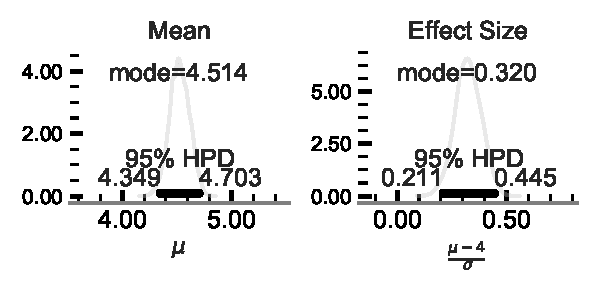
\includegraphics[width=0.67\textwidth]{./hari-code/mean-effect-main.pdf}
 \caption{The posterior density plot for the mean ($\mu$), and the effect size.  The plots show High Posterior Density (HPD) intervals, which represent the region with 95\% of the density. Notice that the HPD interval for $\mu$ is $[4.349, 4,703]$ and excludes 4 (the neutral response value), implying that on average, the response to the comic panel was more persuasive than the text. The figure for the effect size show a moderate effect with mode $0.32$; since the HPD interval $[0.211, 0.445 ]$ excludes 0, we can be confident about the effect.}
 \label{fig:main-experiment-effect}
\end{figure}

\begin{figure}
 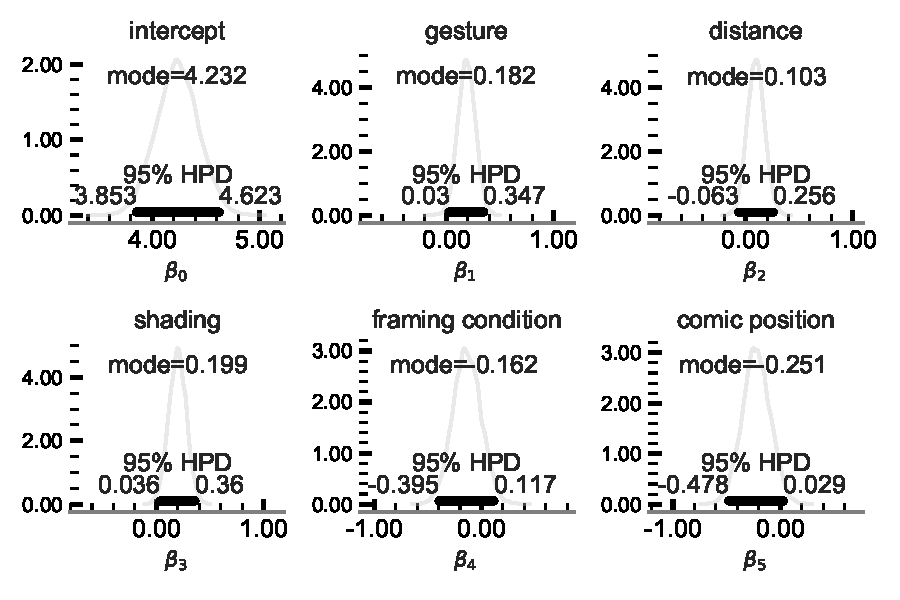
\includegraphics[width=\textwidth]{./hari-code/beta-main.pdf}
 \caption{The posterior density plot for the coefficients ($\beta_i$).  The plots show High Posterior Density (HPD) intervals, which represent the region with 95\% of the density. Notice that the HPD intervals for gesture $[0.03, 0.347]$ (the character gesture) and shading $[0.036, 0.36]$ exclude 0, implying that they have an effect on the response. The HPD intervals for distance between characters, framing condition (positive or negatively framed message) and comic position (comic on the left or on the right of the text) include 0, and thus show no credible effect on the response.}
 \label{fig:beta-main}
\end{figure}
